% Copyright 2005-2016 Airbus-EDF-IMACS-Phimeca
% Permission is granted to copy, distribute and/or modify this document
% under the terms of the GNU Free Documentation License, Version 1.2
% or any later version published by the Free Software Foundation;
% with no Invariant Sections, no Front-Cover Texts, and no Back-Cover
% Texts.  A copy of the license is included in the section entitled "GNU
% Free Documentation License".
\renewcommand{\filename}{docUC_InputWithData_CloudDrawing.tex}
\renewcommand{\filetitle}{UC :  Draw of clouds}

% \HeaderNNIILevel
% \HeaderIILevel
\HeaderIIILevel



\index{Graph!Clouds of points}
\index{Graph!Pairs graph}
\index{View Image}
\index{Graph!Superposition of graphs}



The objective of this Use Case is to draw a cloud of points when points are bidimensional and all the possible pairs of components when the points are of dimension $n>2$.


\requirements{
  \begin{description}
  \item[$\bullet$] one  sample of dimension 2 : {\itshape sample2d}
  \item[type:]  NumericalSample
  \item[$\bullet$] one  sample of dimension $n=4$ : {\itshape sample4d}
  \item[type:]  NumericalSample
  \end{description}
}
             {
               \begin{description}
               \item[$\bullet$] the files containing the cloud graph
               \item[type:] files in all possible formats
               \end{description}
             }

             \textspace\\
             Python script for this UseCase :

             \inputscript{script_docUC_InputWithData_CloudDrawing}

             \textspace\\



             Figure (\ref{cloud2}) draws the superposition of two clouds of dimension 2 and size 1000, realizations of :
             \begin{itemize}
             \item a Normal distribution with $\vect{0}$ mean, unit standard deviation and independant components,
             \item a Normal distribution with unit-mean,  unit-standard deviation and independant components.
             \end{itemize}

             Figure (\ref{cloud2}) draws all the possible pairs of components from a sample of dimension 4 and size $N=500$, generated by a Normal distribution with correlation matrix $\mat{R} (C_{ij})_{ij}$ such that the components 1 and 2 are correlated with $R_{12} = 0.8$ and the components 3 and 4 are correlated with $R_{34} = -0.7$.

             \begin{figure}[H]
               \begin{center}
                 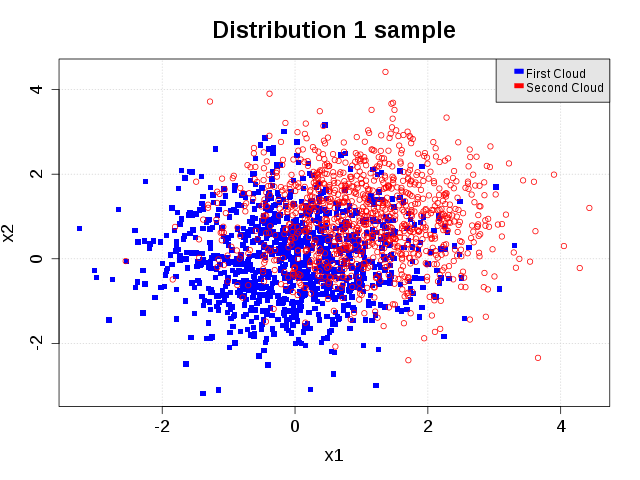
\includegraphics[width=10cm]{Figures/cloud2.png}
               \end{center}
               \caption{Superposition of two normal numerical sample of dimension 2.}
               \label{cloud2}
             \end{figure}


             \begin{figure}[H]
               \begin{center}
                 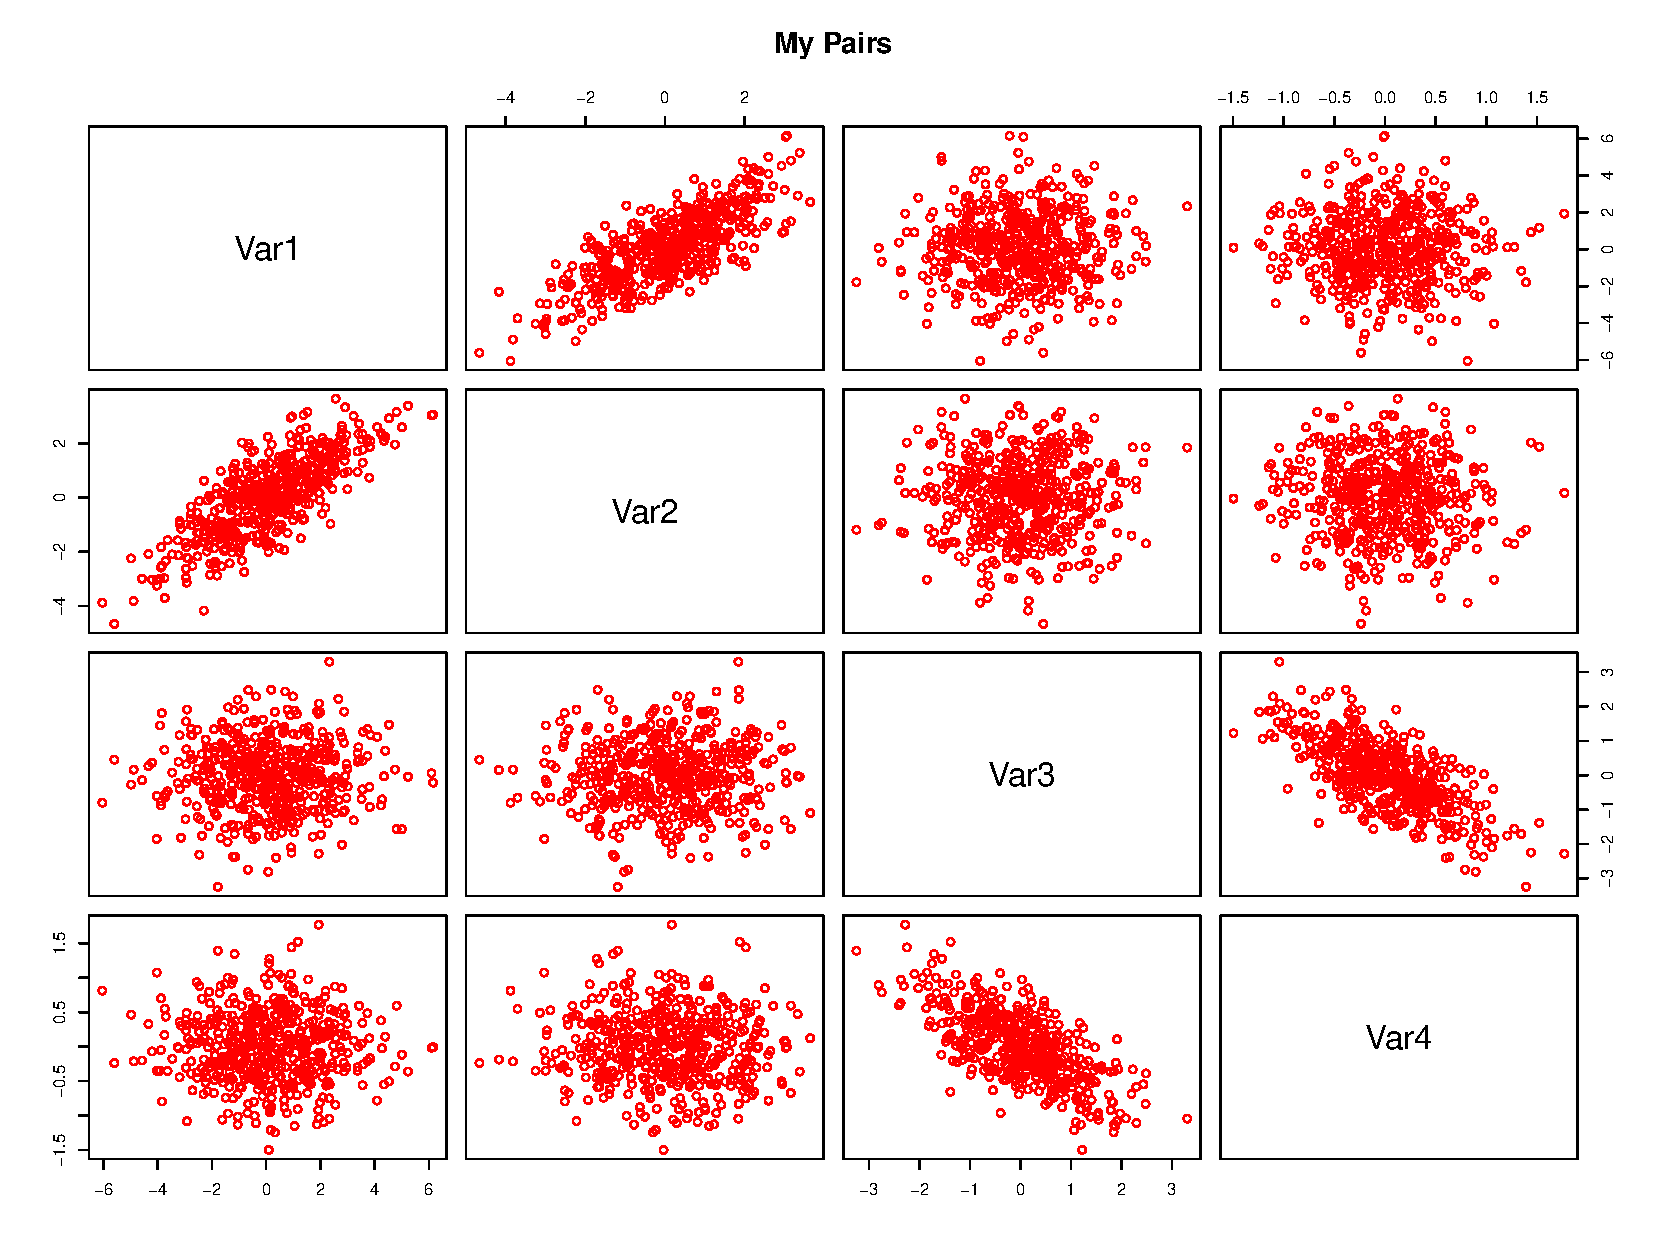
\includegraphics[width=10cm]{Figures/pairs.pdf}
               \end{center}
               \caption{Pairs graph for a sample of dimension 4.}
               \label{cloud2}
             \end{figure}
